% !TEX root = main.tex

\chapter{Existing experimental system}
The work developed in this thesis lies on top of an existing experiment. In this chapter we are going to describe the essential parts of the already existing setup on top of which the addressing system has been build. Calcium-40 ions are used in the experiment, the implementation of several techniques for
trapping and manipulating these ions are discussed. Furthermore, the addressing setup utilizes 393nm light, the laser emitting this light was already installed and used, thus that setup is presented. The experiment can be controlled remotely via computers, an overview of how it is implemented and how it works is also given.

\section{Ion trap and key techniques}
\subsection{Calcium Ions}
In choosing the appropriate ion to trap, one looks first of all for simplicity, which means choosing an element with one single electron in the most outer orbital.
This fact limits the choice to the second group of the periodic table, many of these elements has been successfully trapped: beryllium [], barium [], strontium [], and calcium [].
The latter has been chosen for this experiment, as calcium has transitions easily accessible with commercial diode and titanium-sapphire lasers. The most abundand isotope of calcium is calcium-40, which is a common choice, but not the only one []. Nevertheless, $^{40}\text{Ca}^+$ ions were our choice. In figure \ref{calciumscheme} the level scheme of the only electron in the outer shell is presented. A single ground state is present $\text{S}_{1/2}$ with no hyperfine structure as $^{40}\text{Ca}^+$ does not posses a nuclear spin. There are two short lived excited states ($\sim 7$ ns): $\text{P}_{1/2}$, and $\text{P}_{3/2}$ which are accessible with dipole transitions. These states have different decay channel, for $\text{P}_{1/2}$
the branching ratios are $6\%$ to $\text{D}_{3/2}$, and $94\%$ back to the ground state. For  $\text{P}_{3/2}$ there is a probability of $5.3\%$ to decay to   $\text{D}_{5/2}$, $0.6\%$ to go to  $\text{D}_{3/2}$ and $94\%$ to return to  $\text{S}_{1/2}$. Due to the short lifetimes of these two states, they are suitable for laser cooling and state detection, while the states $\text{D}_{3/2}$ and $\text{D}_{5/2}$
are metastable ($\sim 1$ s) since accessible with electric quadrupole transition. Since the lifetime of the D states are much greater than typical coherence time, they can encode a stable qubit and manipulated without worrying about dissipative process. Table () summarizes the properties of the states, and details about the different transition.

\begin{tabular}{c c c c c}
 \toprule
    {Transition} & {wavelength (nm)} & {Decay rate $\Gamma$} & {Type} & {Use} \\ \midrule
   16.128 & 1.402 & 1.373 & -146.6 & -137.6 \\
     3.442  & 0.299 & 0.343 & 133.2  & 152.4  \\
     1.826  & 0.159 & 0.119 & 168.5  & -161.1 \\
     0.993  & 0.086 & 0.08  & 25.6   & 90     \\ \midrule
   1.29   & 0.112 & 0.097 & -175.6 & -114.7 \\
     0.483  & 0.042 & 0.063 & 22.3   & 122.5  \\
     0.766  & 0.067 & 0.039 & 141.6  & -122   \\
     0.624  & 0.054 & 0.04  & -35.7  & 90     \\ \midrule
   0.641  & 0.056 & 0.045 & 133.3  & -106.3 \\
     0.45   & 0.039 & 0.034 & -69.4  & 110.9  \\
     0.598  & 0.052 & 0.025 & 92.3   & -109.3 \\ \bottomrule
\end{tabular}

\begin{figure}
\centering
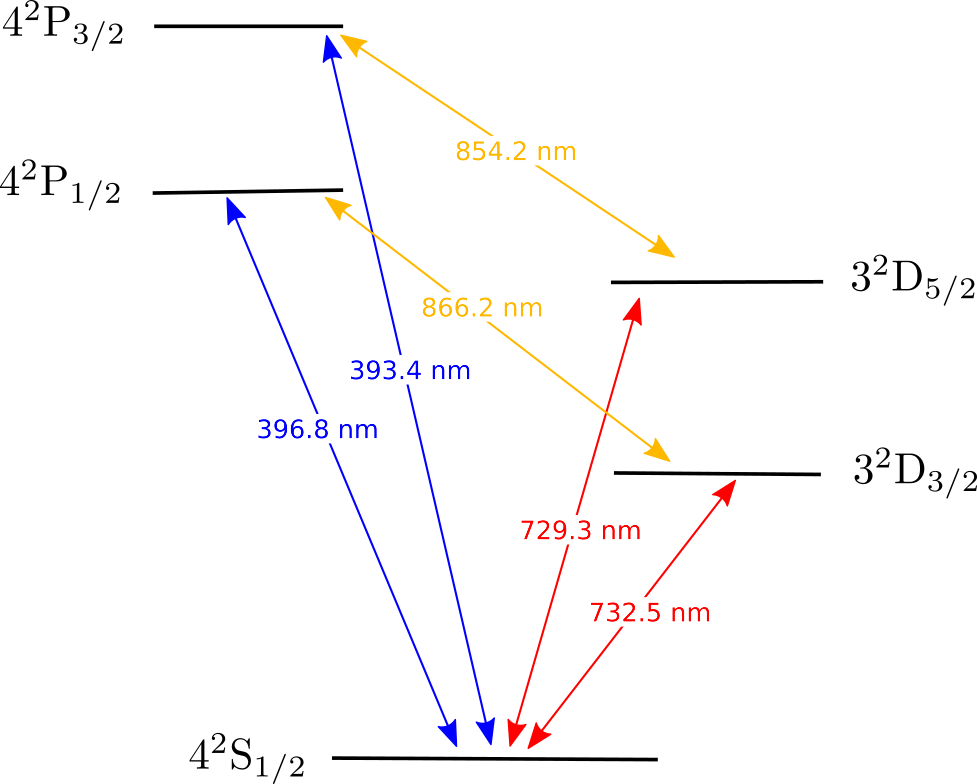
\includegraphics[width = .6 \textwidth]{calciumscheme}
\caption{Level scheme of $^{40}\text{Ca}^+$.}
\label{calciumscheme}
\end{figure}


\subsection{Trapping, cooling, and state readout}
- How this stuff is implemented
\subsection{Photon generations}
- Cavity enhanced Raman transition
\section{393nm laser}
\section{Experiment control}
